\documentclass{article}
\usepackage{pgfplots}
\pgfplotsset{compat=1.18}

\begin{document}

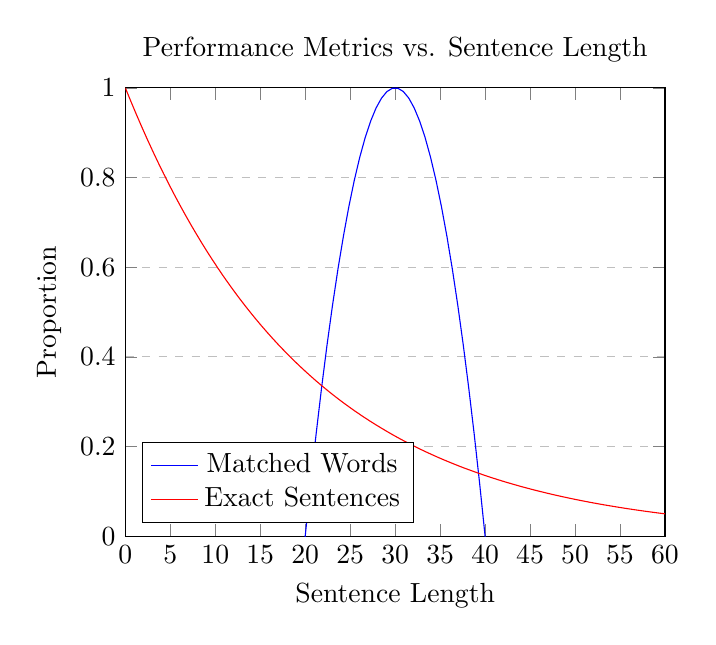
\begin{tikzpicture}
    \begin{axis}[
        title={Performance Metrics vs. Sentence Length},
        xlabel={Sentence Length},
        ylabel={Proportion},
        xmin=0, xmax=60,
        ymin=0, ymax=1,
        xtick={0,5,...,60},
        ytick={0,0.2,...,1},
        legend pos=south west,
        ymajorgrids=true,
        grid style=dashed,
    ]
    
    \addplot[
        color=blue,
        mark=none,
        domain=0:60,
        samples=100,
    ] {1 - 0.01 * (x - 30)^2};
    \addlegendentry{Matched Words}
    
    \addplot[
        color=red,
        mark=none,
        domain=0:60,
        samples=100,
    ] {exp(-0.05 * x)};
    \addlegendentry{Exact Sentences}
    
    \end{axis}
\end{tikzpicture}

\end{document}